%\documentclass[a4paper]{article}
%\usepackage[utf8]{inputenc}
%\usepackage{amsthm}             % Definitions and such
%\usepackage{amssymb}            % R for space and such
%\usepackage{amsmath}
%\usepackage[a4paper]{geometry}
%
%\title{LINMA2471 : Optimization models and models : course 6 (28/10/2015)}
%\author{Renaud Dufays, Antoine Durviaux \& Leïla Van Keirsbilck}
%\date{Octobre 2015}
%
%\usepackage{natbib}
%\usepackage{graphicx}
%\usepackage{framed}
%\usepackage{tikz}
%\usepackage{float}
%\usetikzlibrary{arrows}
%\usetikzlibrary{decorations.markings}
%
%
%\begin{document}
%
%\maketitle

\subsection{Reminders}
\textcolor{red}{subsection to move}

\begin{definition}
Let $\mathcal{C}$ be a closed convex set and f a differentiable function. We consider the constraint problem $\underset{x\in \mathcal{C}}{\min}\ f(x)$. A \textbf{stationary point} is a point $x^*$ such that
\begin{equation*}
\langle \nabla f(x^*), x-x^* \rangle \ \geq\ 0 \ \ \ \ \forall x \in \mathcal{C}
\end{equation*}
\end{definition}

Intuitively, that means that all possible errors $x-x^*$ are in opposite direction with $-\nabla f$. A schema of the situation is shown on figure \ref{tik1}.
\begin{figure}[H]
\centering
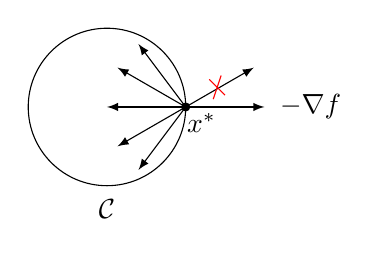
\begin{tikzpicture}
\draw (0,0) circle (1);
\draw[fill = black] (1,0) circle (0.05);
\draw (0,-1.3) node{$\mathcal{C}$};
\draw (1.2,-0.2) node{$x^*$};
\draw[>=latex,->] (1,0) -- (2,0) node{$\ \ \ \ \ \ \ \ \ \ -\nabla f$};
\draw[>=latex,->] (1,0) -- (1.866025403784439,0.5);
\draw[>=latex,->] (1,0) -- (0,0);
\draw[>=latex,->] (1,0) -- (0.133974596215561,0.5);
\draw[>=latex,->] (1,0) -- (0.133974596215561,-0.5);
\draw[>=latex,->] (1,0) -- (0.4,0.8);
\draw[>=latex,->] (1,0) -- (0.4,-0.8);
\draw[red] (1.5,0.15) -- (1.3,0.35);
\draw[red] (1.35,0.1) -- (1.45,0.4);
\end{tikzpicture}
\caption{Example of a stationnary point $x^*$.}
\label {tik1}
\end{figure}

\begin{example}
\begin{leftbar}
 $\mathcal{C} = \{x \in \mathbb{R}^n: x_i \ge 0\}$ (nonnegative orthant)
\begin{align*}
&x^* \; \text{stationnary iff} \; \sum_i \left[\nabla f(x^*)\right]_i \left[x_i - x_i^*\right] \ge 0\ \ \ \forall x\ge 0\\
&x^* \; \text{stationnary iff either} \; [\nabla f(x^*)]_i=0\\ 
&\phantom{x^* \; \text{stationnary iff eith}}\text{or} \; [\nabla f(x^*)]_i>0 \; \text{and} \; x_i^*=0 \; \forall \; i
\end{align*}
Indeed, as $\sum_i [x_i - x_i^*] \ge 0$ for all $x\ge0$,  $[\nabla f(x^*)]_i$ must be $\ge 0$.
If not, we could choose a very large $x_i$ for this component and have a negative sum.
\end{leftbar}
\end{example}

\begin{example}
\begin{leftbar}
It also works easily for $\mathcal{C} = \{x|\sum_{i}x_i=1\}$ which is a kind of budget constraint. In that case, it is possible to show that $[\nabla f(x^*)]_i = \lambda \; \forall i$. That means that all the gradient components are equal to each other, or economically speaking that the marginal costs are equal to each other. At the optimum, the marginal cost is equal for each component, it does not matter which one you lower.
\end{leftbar}
\end{example}

\begin{example}
\begin{leftbar}
(not treated) The Euclidian bowl.
\end{leftbar}
\end{example}


%\paragraph{Projected gradient method ($f\in C_L^{1,1}$)}~~\\
%\newline
%\hspace*{2cm}
%\fbox{\parbox{6cm}{
%~~Given $x_0$, $L$, $k=0$ \\
%\begin{tabular}{l|l}
%Repeat & $x_{k+1} = P_C[x_k - \frac{1}{L}\nabla f(x_k)]$\\
 %& $k \leftarrow k+1$
 %\end{tabular}}} 


\subsection{Gradient mapping for constrained problems}

\begin{definition}
For some $M>0$, the \textbf{gradient mapping} $G_M^Cf(x)$ is the unique vector satisfying 
\begin{equation*}
x - \frac{1}{M}G_M^Cf(x) = P_C\left[x - \frac{1}{M}\nabla f\right]
\end{equation*}
\end{definition}

The role of the gradient mapping is similar to the one of the gradient in the non-constraint case. Notice that if we take $\mathcal{C} = \mathbb{R}^n$, then $G_M^{\mathbb{R}^n}f(x) = \nabla f(x)$. An illustration of the gradient mapping is given in Figure \ref{tik2}.

\begin{figure}[H]
\centering
	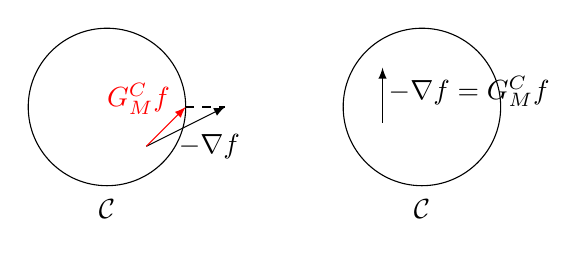
\begin{tikzpicture}
    \draw (0,0) circle (1);
    \draw (0,-1.3) node{$\mathcal{C}$};
    \draw[>=latex,->] (0.5,-0.5) -- (1.5,0);
    \draw (1.3,-0.5) node{$-\nabla f$};
    \draw[red] (0.4,0.1) node{$G_M^C f$};
    \draw[>=latex,->,red] (0.5,-0.5) -- (1,0);
    \draw[dashed] (1,0) -- (1.5,0);
    \draw (4,0) circle (1);
    \draw (4,-1.3) node{$\mathcal{C}$};
    \draw[>=latex,->] (3.5,-0.2) -- (3.5,0.5);
    \draw (4.6,0.2) node{$-\nabla f = G_M^C f$};
    \end{tikzpicture}
\caption{Illustration of gradient mapping.}
\label {tik2}
\end{figure}

The gradient method becomes, in the case of constraint problems :

\begin{lstlisting}[mathescape,caption=Gradient Method - Constrained Problem]
Given $x_0$, $L$, $k=0$
Repeat
$\qquad   x_{k+1} = P_C[x_k - \frac{1}{L}G_M^C f(x_k)]$
$\qquad  k \leftarrow k+1$
\end{lstlisting}


\begin{property}
For any $M>0$, we have $x^*$ stationary iff $G_M^C f(x^*)=0$
\end{property}

\begin{property}
Given $f \in C^{1,1}_L$, and letting $x^+ = x - \frac{1}{L}G^C_L f(x)$ be the next step, we have
\[
    f(x) - f(x^+) \ge \frac{\left\|G_L^C f(x)\right\|^2}{2L}
\]
\end{property}


\begin{theorem} Using those properties, we obtain that for $f \in C_L^{1,1}$, the projected gradient method gives
\begin{equation*}
\min_{0\leq i \leq N} \left\|G_L^C f(x_i)\right\| \leq \sqrt{\frac{2(f(x_0) - f(x^*))}{L(N+1)}}
\end{equation*}
\end{theorem}

We have a stronger result in the case of a convex $f$, as stated by the following theorem.
\begin{theorem}
Let $f \in F_L^{1,1}$. For any iterate $x_N$ and any $x$,
\begin{equation*}
f(x_N) - f(x^*) \leq \frac{M\left\|x_0 - x^*\right\|^2}{2N}
\end{equation*}
\end{theorem}


The projected gradient method is quite slow because it is in $\mathcal{O}(\frac{1}{N})$ but also because projection can be complicated. Indeed, projection can be hard to compute if $\mathcal{C}$ is too complex.

\begin{example}
\begin{leftbar}
If $\mathcal{C}=\{x\ge0\}$ this is easy because $[P_C(x)]_i=\left\lbrace
\begin{array}{ll}
x_i & \mbox{if $x_i \ge 0$}\\
0 & \mbox{if $x_i < 0$}
\end{array}
\right.$
\end{leftbar}
\end{example}

\begin{example}
\begin{leftbar}
If $\mathcal{C}=\{x|Ax=b\}$ is a subspace, this is expensieve. We have indeed to solve a linear system, which is $\mathcal{O}(n^3)$.
\end{leftbar}
\end{example}

\begin{example}
\begin{leftbar}
If $\mathcal{C}=\{x|Ax\leq b\}$ is a polyhedron, this is even more expensive : the projection problem has to be written as a minimization of the distance (quadratic programming). We could also use a theorem that separates the problem on each facet of the polytope.
\end{leftbar}
\end{example}


\subsection{Acceleration gradient [Nesterov 1983]}


\begin{lstlisting}[mathescape,caption=Acceleration gradient]
Given $f \in C^{1,1}_L$, $x_0$, $L$, $k=0$ and $x_{-1}=x_0$
Repeat 
$\qquad y_k = x_k + \beta_k (x_k - x_{k-1})$
$\qquad x_{k+1} = P_C[y_k - \frac{1}{L}\nabla f(y_k)]$
$\qquad k \leftarrow k+1$
\end{lstlisting}

The first step is called an extrapolation step whereas the second is called a gradient step. Note that $y_k$ is not always in $\mathcal{C}$. The idea is to recycle the previous work because $(x_k - x_{k-1})$ will be close to the gradient.

\begin{theorem}
For $\beta_k=\frac{k-1}{k+2}$, we have
\begin{equation*}
f(x_N) -  f(x^*) \leq \frac{2L\left\|x_0 - x^*\right\|^2}{(N+1)^2}
\end{equation*}
\end{theorem}

It can be proved that this rate of $\frac{1}{N^2}$ is not improvable. Accelerated gradient is thus a sublinear method (slower than linear). While the gradient method is really robust, the accelerated method is extremely sensitive. Note that $\beta_k$ goes to 1 as k goes to infinity. An example is the Huber function : on the linear part, the steps increase in a quadratic way.\\

\textbf{Linear convergence (to zero) :} $1, \rho, \rho ^2, \rho ^3, \rho ^4, \rho ^5, ... $ with $\rho < 1$. If we restrict the class of functions to \textbf{strongly convex}, we can get linear convergence.\\

\begin{definition}
Given $\mu>0$, f is $\mu$-\textbf{strongly convex} iff
\begin{equation*}
f(\lambda x + (1-\lambda)y)\leq \lambda f(x) + (1-\lambda)f(y) - \frac{\mu}{2}\lambda (1-\lambda)\left\|x - y\right\|^2
\end{equation*}
\end{definition}

A strongly-convex function can be viewed as a function that has no flat part.

\begin{proposition}
If $f \in C^2$ then f is $\mu$-strongly convex iff for all $x$ 
\[
    \lambda_{min}(\nabla^2f(x))\ge \mu
\]
\end{proposition}


\begin{lemma}
For any strongly convex function, we have
\begin{equation*}
\left\|x - x^*\right\|^2 \leq \frac{2}{\mu}[f(x) - f(x^*)]
\end{equation*}
That means that if I decrease the error on the function value, automatically I decrease the distance to the solution. Using previous results, we obtain :
\begin{equation*}
\left\|x_N - x^*\right\|^2 \leq \frac{2}{\mu}\frac{L\left\|x_0 - x^*\right\|^2}{2N} = \frac{L}{\mu}\frac{\left\|x_0 - x^*\right\|^2}{N}
\end{equation*}
\end{lemma}

$\frac{L}{\mu}$ is called the condition number.


\textbf{Remark:} The accelerated gradient method gives better results if we restart the method after a certain number of iteration. For example, if the squared norm of the error is divided by 5 after $N = 10$ iterations, it will be divided by 10 after $N = 20$ iterations. But if we restart the method after 10 iterations and make 10 new iterations, the square norm of the error will be divided by 25 although we made a total of 20 iterations in both cases. A result that is not proven here is that the optimal number of iterations after which the method should be restarted is $\frac{L}{\mu}\text{e}$. In this case, the method is linearly convergent and we have :
\[
    \left\|x_N - x^*\right\|^2 \leq \left(1-\frac{1}{\text{e}\frac{L}{\mu}}\right)\left\|x_0 - x^*\right\|^2
\]

\textbf{\textcolor{red}{UNTIL HERE: form controlled, contained te be controlled}}
%\end{document}
